\documentclass[a4paper,14pt]{article}
\usepackage{float}
\usepackage{extsizes}
\usepackage{amsmath}
\usepackage{amssymb}
\everymath{\displaystyle}
\usepackage{geometry}
\usepackage{fancyhdr}
\usepackage{multicol}
\usepackage{graphicx}
\usepackage[brazil]{babel}
\usepackage[shortlabels]{enumitem}
\usepackage{cancel}
\usepackage{textcomp}
\columnsep=2cm
\hoffset=0cm
\textwidth=8cm
\setlength{\columnseprule}{.1pt}
\setlength{\columnsep}{2cm}
\renewcommand{\headrulewidth}{0pt}
\geometry{top=1in, bottom=1in, left=0.7in, right=0.5in}

\pagestyle{fancy}
\fancyhf{}
\fancyfoot[C]{\thepage}

\begin{document}
	
	\noindent\textbf{8FMA72 - Matemática} 
	
	\begin{center}Intersecções (Versão estudante)
	\end{center}
	
	\noindent\textbf{Nome:} \underline{\hspace{10cm}}
	\noindent\textbf{Data:} \underline{\hspace{4cm}}
	
	%\section*{Questões de Matemática}
	
	
    \begin{multicols}{2}
    	\noindent Para encontrar as coordenadas do(s) ponto(s) de intersecção(ões) entre os gráficos de duas relações, basta resolvermos o sistema formado por suas equações. \\
    	\noindent Para encontrar as coordenadas do(s) ponto(s) de intersecção(ões) de um gráfico com os eixos coordenados, fazemos as substituições $x = 0$ e, posteriormente, $y = 0$ na expressão fornecida.
    	\noindent\textsubscript{~---------------------------------------------------------------------------}
		\begin{enumerate}
			\item Encontre as coordenadas dos pontos de intersecção dos gráficos das relações dadas por:
			\begin{enumerate}[a)]
				\item $x^2 + y^2 = 12$ e $y = x$. \\\\\\\\\\\\\\\\\\\\\\\\\\\\\\\\\\\\
				\item $3x + y - 5 = 0$ e $2x - 3y + 4 = 0$.
				\\\\\\\\\\\\\\\\\\\\\\\\\\\\\\\\\\\\
				\item $x \cdot y = -1$ e $y = -x^2$
				\\\\\\\\\\\\\\\\\\\\\\\\\\\\
			\end{enumerate}
		    \item Encontre os pontos de intersecção dos gráficos das seguintes relações com os eixos coordenados:
		    \begin{enumerate}[a)]
		    	\item $y = x + 7$ \\\\\\\\\\\\\\\\\\\\\\
		    	\item $3y - 4x + 6 = 0$ \\\\\\\\\\\\\\\\\\\\\\
		    	\item $y = x^2 + 3x - 10$ \\\\\\\\\\\\\\\\\\\\\\
		    \end{enumerate}
	        \item Encontre a área da região determinada pelo eixo das ordenadas e pelas relações dadas por $y = -3x + 4$ e $y - x = 0$. \\\\\\\\\\\\\\\\\\\\\\\\\\\\\\\\
	        \item Encontre os pontos de intersecção dos gráficos das relações dadas por:
	        \begin{enumerate}[a)]
	        	\item $x + 2y = 6$ e $3x - y = 4$  \\\\\\\\\\\\\\\\\\\\\\\\\\\\\\
	        	\item $x^2 + y^2 = 5$ e $x^2 + y^2 - 6x = -1$ \\\\\\\\\\\\\\\\\\\\\\\\\\
	        	\item $x^2 = y^2$ e $4x + y = 5$ \\\\\\\\\\\\\\\\\\\\\\\\\\
	        	\item $x^2 + 4y^2 = 13$ e $3x^2 - y^2 = 0$ \\\\\\\\\\\\\\\\\\\\\\\\
	        \end{enumerate}
            \item Encontre os pontos de intersecção dos gráficos das relações dos itens $a$ e $b$ do exercício anterior com os eixos coordenados. \\\\\\\\\\\\\\\\\\\\\\\\\\
            \item Na figura, considere os gráfios das relações $f(x) = ax + b$ e $g(x) = mx + n$. Se $P = \bigg(\frac{20}{7}; \frac{6}{7}\bigg)$, o valor de $\frac{a + n}{b \cdot m}$ é: 
            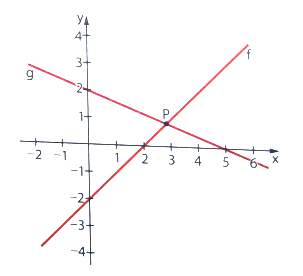
\includegraphics[width=1\linewidth]{imagens_8FMA72/imagens1}
        \end{enumerate}
    $~$ \\ $~$ \\ $~$ \\ $~$ \\ $~$ \\ $~$
    \end{multicols}
\end{document}